%                                                                 aa.dem
% AA vers. 9.1, LaTeX class for Astronomy & Astrophysics
% demonstration file
%                                                       (c) EDP Sciences
%-----------------------------------------------------------------------
%
%\documentclass[referee]{aa} % for a referee version
\documentclass[onecolumn]{aa} % for a paper on 1 column  
%\documentclass[longauth]{aa} % for the long lists of affiliations 
%\documentclass[letter]{aa} % for the letters 
%\documentclass[bibyear]{aa} % if the references are not structured 
%                              according to the author-year natbib style

%
%\documentclass{aa}  

%
%\usepackage{deluxetable}
\usepackage{graphicx}
%%%%%%%%%%%%%%%%%%%%%%%%%%%%%%%%%%%%%%%%
\usepackage{txfonts}
%%%%%%%%%%%%%%%%%%%%%%%%%%%%%%%%%%%%%%%%
%\usepackage[options]{hyperref}
% To add links in your PDF file, use the package "hyperref"
% with options according to your LaTeX or PDFLaTeX drivers.
%
\begin{document} 


   \title{Core-collapse supernova 56Ni masses lower limits}

   %\subtitle{I. subtitle}

 \author{Nicol\'as~Meza\inst{1} \and J.P.~Anderson\inst{1} }

   \institute{European Southern Observatory, Alonso de C\'ordova 3107, Casilla 19, Santiago, Chile}

   \date{Received ; accepted }

% \abstract{}{}{}{}{} 
% 5 {} token are mandatory
 
  \abstract
  % context heading (optional)
  % {} leave it empty if necessary  
   {The mass of radioactive material is an important parameter in the explosion and the optical emission of any Supernova type. Recent work has compiled and obtained the distribution of nickel , showing that the distribution of stripped enveloped core-collapse supernovae (Stripped-CCSNe) is highly incompatible with the hydrogen rich supernovae (type II-SNe) distribution.}{Measure the $^{56} Ni$ for a significant sample of Stripped-CCSNe in a uniform manner to confirm the Stripped/Hydrogen-rich discrepancy}{We compiled a sample of well observed Stripped-CCSNe and measured $^{56} Ni$ masses from different methods proposed in the literature, namely the Arnett's rule, from the radioactive tail and the new prescription by Khatami \& Kasen.}{Neither of Khatami prescription or lower limits from the radioactive tail are sufficient to make the distribution of Stripped-CCSNe statistically compatible with the same from type-II SNe.}{Conclusions}

   \keywords{supernova - general  }

   \maketitle
%
%-------------------------------------------------------------------

\section{Introduction}

\section{Data and sample selection} 
\label{sec:data}

\begin{figure}[ht!]
 \centering
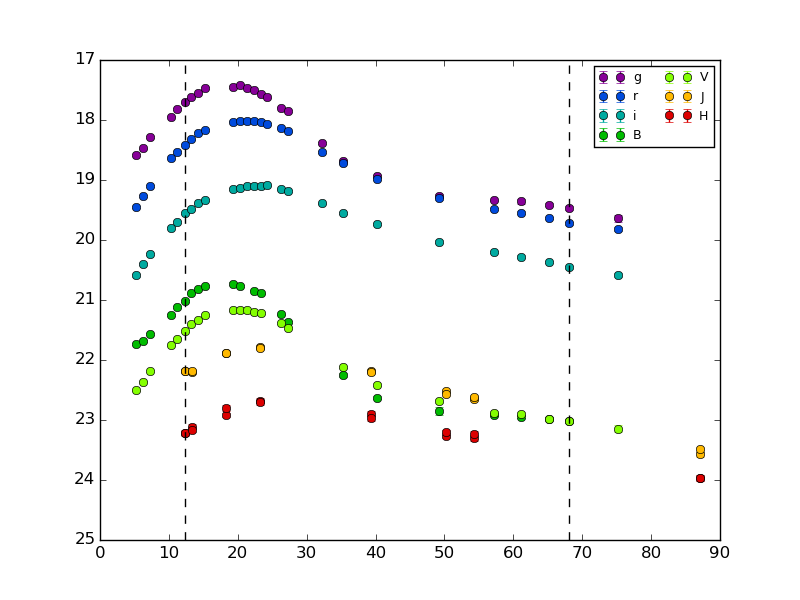
\includegraphics[width=\linewidth]{plots/SN2004ex_lcs.png}
\caption{Light curves (in arbitrary magnitude scales) for SN2004ex. A couple of dashed lines marks the boundaries where the bolometric light curves are built after interpolation.\label{fig:lc_example}}
\end{figure}

\section{Analysis}
\label{sec:analysis}

\begin{figure}[ht!]
 \centering
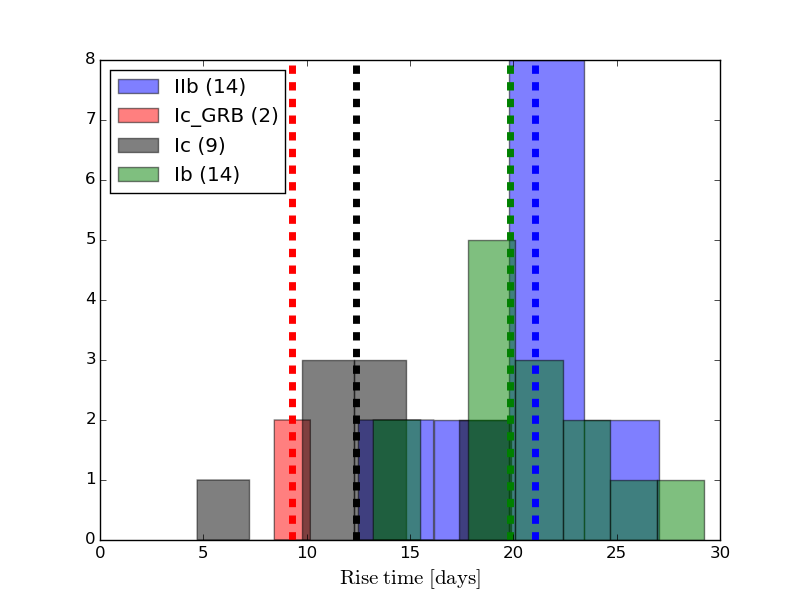
\includegraphics[width=\linewidth]{plots/BVRIYJH_rise_hist_subtypes.png}
\caption{Rise time distribution of our BVRIYJH sample. Each SN subtype is color labeled and a vertical line of the same color is used to mark the median of that distribution.\label{fig:rise_dist}}
\end{figure}


\begin{figure}[ht!]
 \centering
\includegraphics[width=\linewidth]{plots/SED_lam_BgVriYJH_3_1.png}
\caption{Example of the temporal evolution of a supernova SED. Each SED is color coded by the time since explosion. Each filters is labeled with a dashed vertical line and the name of the filter is at the top.\label{fig:SED_example}}
\end{figure}



\subsection{Bolometric light curves}

\begin{figure}[ht!]
 \centering
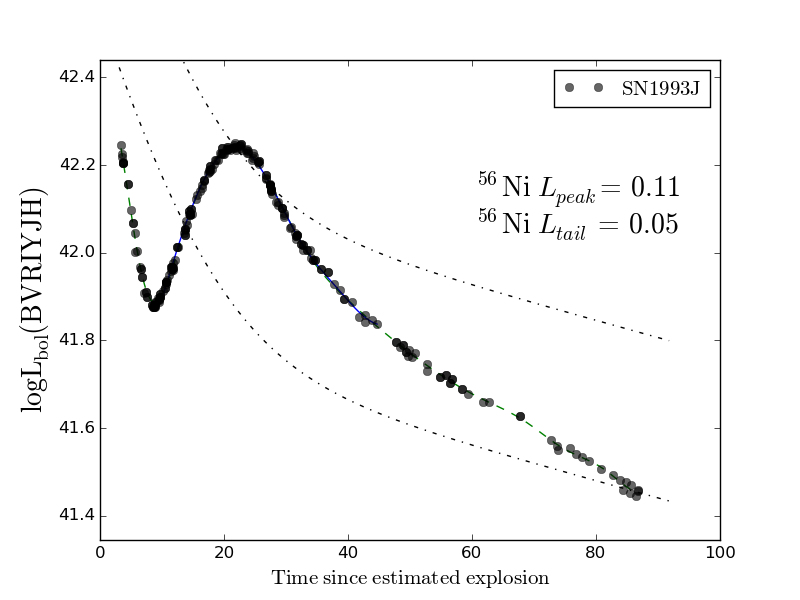
\includegraphics[width=\linewidth]{plots/SN1993J_BVRIYJH_Lbol.png}
\caption{Example of a very well sampled BVRIYJH bolometric light curve. Dashed lines marks the 56Co decay, assuming an initial 56Ni mass given by the Arnett rule at peak and a lower limit given by the tail, assuming full trapping.\label{fig:bol_example}}
\end{figure}

\subsection{Methods to measure Nickel masses}

\subsection{Systematics}
\begin{figure}[ht!]
 \centering
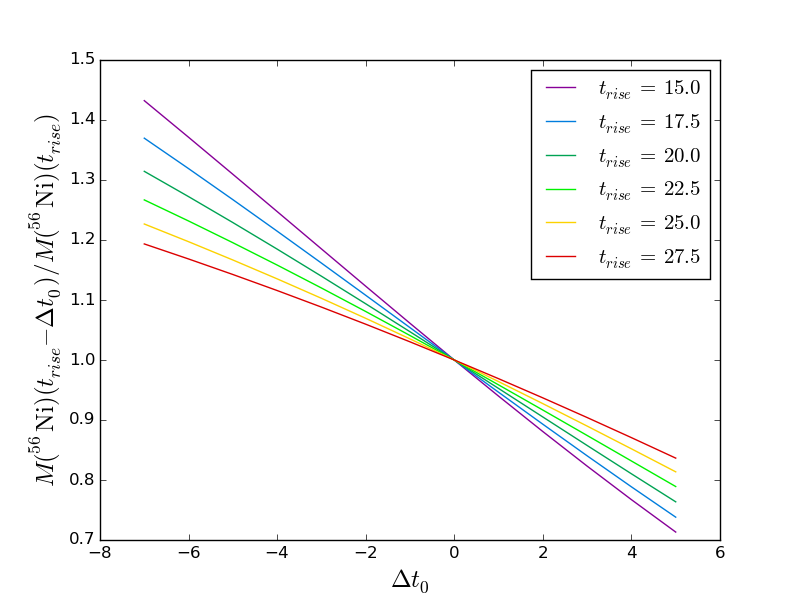
\includegraphics[width=\linewidth]{plots/peak_shift.png}
\caption{Fractional variation of the nickel mass measurement using the Arnett rule, as a function of the rise time variation in days. Color labeled are the curves for different initial rise times. The shorter the real rise time the more the nickel mass is affected by the unknown explosion epoch.\label{fig:peak_shift}}
\end{figure}

\begin{figure}[ht!]
 \centering
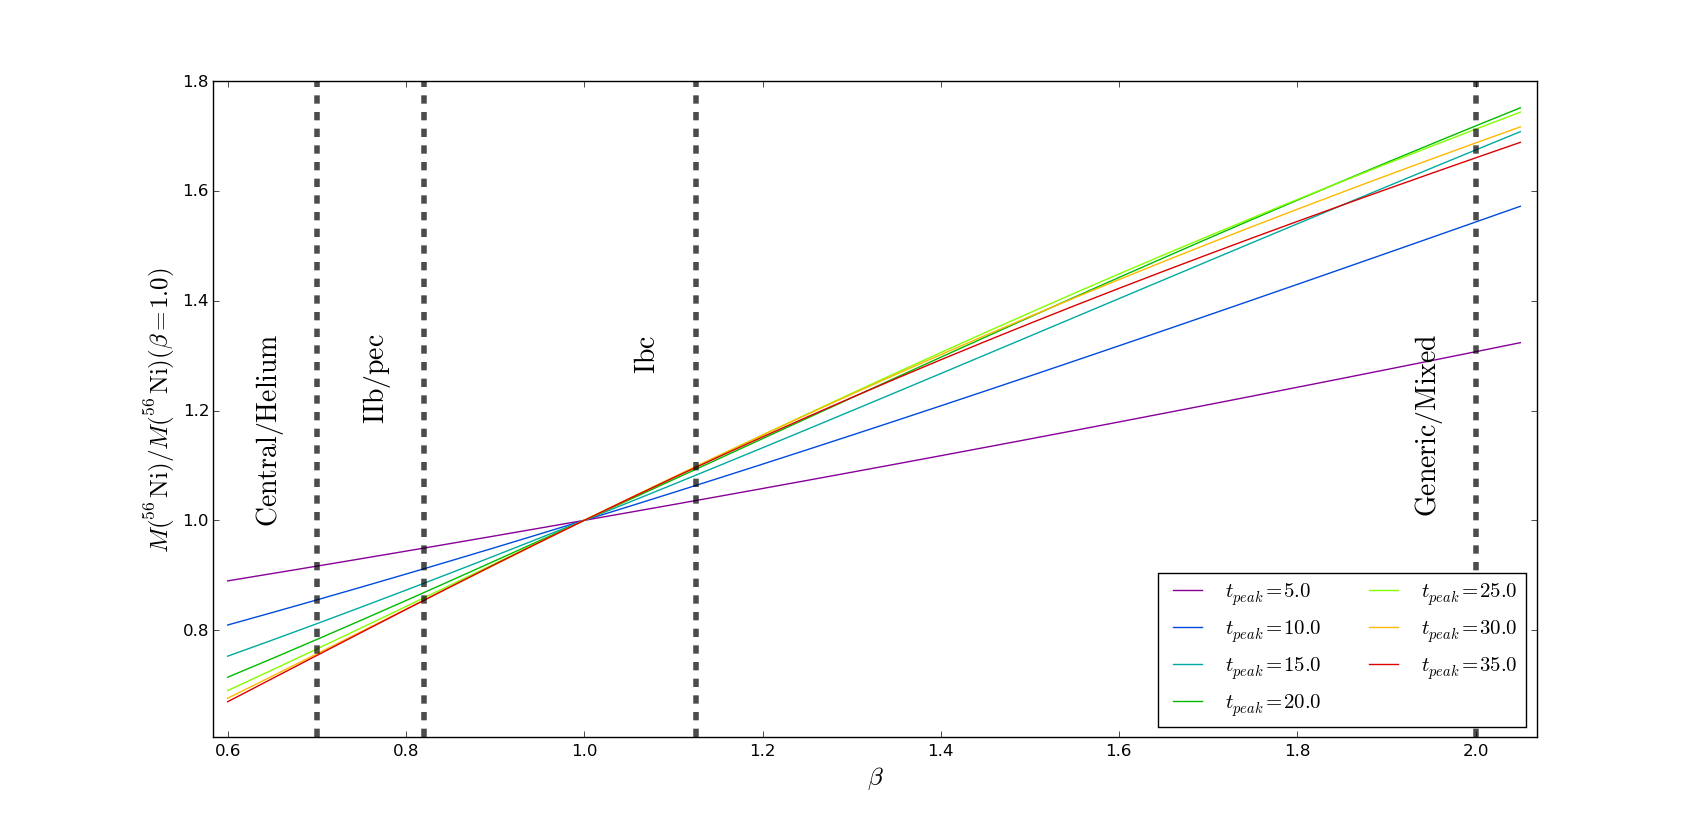
\includegraphics[width=\linewidth]{plots/Khatami_beta.png}
\caption{Fractional Variation of the nickel mass measurement using the Khatami+18 prescription, as a function of the $\beta$ parameter ($\beta=1$ is equivalent to the Arnett rule). Color labeled are the curves for different initial rise times. We mark as dashed black lines reference beta values from different progenitor structures from Khatami+18.\label{fig:khatami_shift}}
\end{figure}

\section{Results}

\begin{figure}[ht!]
 \centering
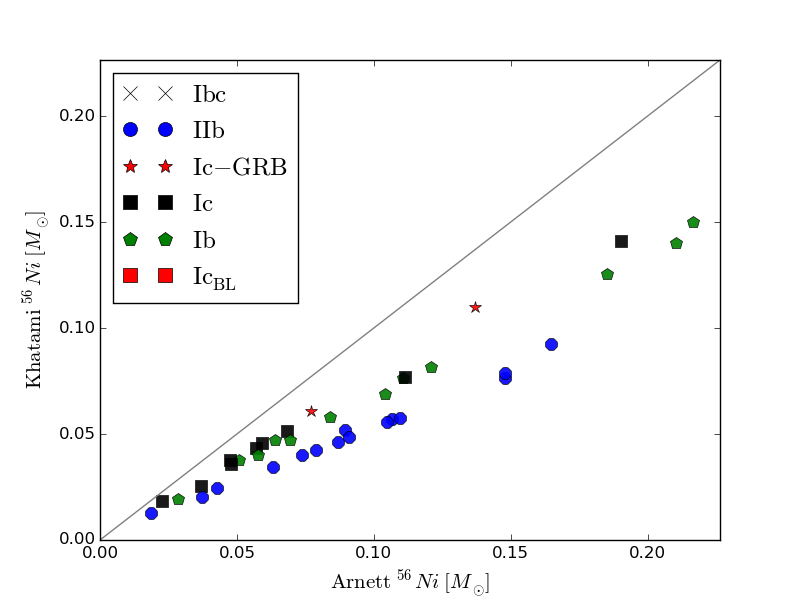
\includegraphics[width=\linewidth]{plots/Arnett_Khatami_BVRIYJH.png}
\caption{Comparison of the 56Ni masses as measured by the Arnett's rule and the Khatami+18 prescription. Each marker is labeled according to each SNe type.  We used the reccomended $\beta$ values for a type IIb/Ibc mixing of 0.82 and $9/8$, respectively. \label{fig:Ni56_comp}}
\end{figure}

\begin{figure}[ht!]
 \centering
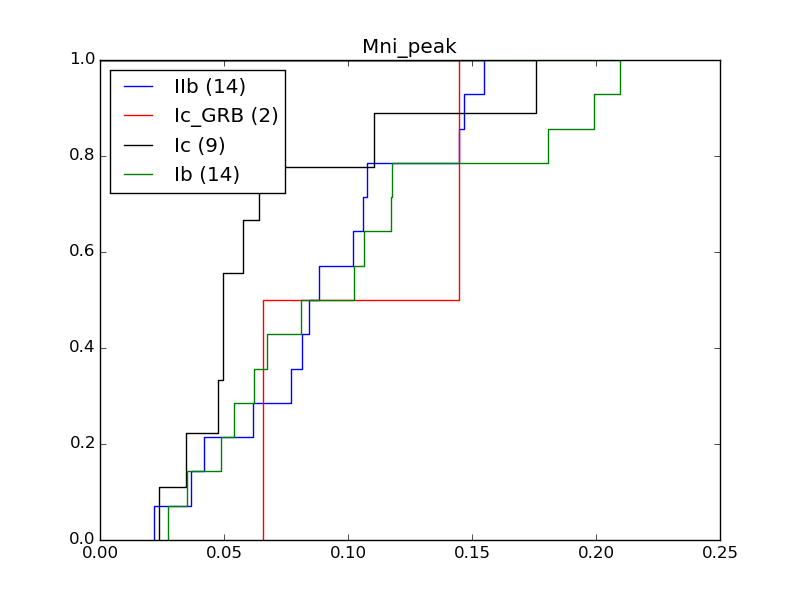
\includegraphics[width=\linewidth]{plots/Mni_peak_hist_subtypes.png}
\caption{Final distribution of 56Ni, using the Arnett's rule, for our BVRIYJH sample of SNe, divided by SN subtypes.\label{fig:hist_subtypes}}
\end{figure}

\begin{figure}[ht!]
 \centering
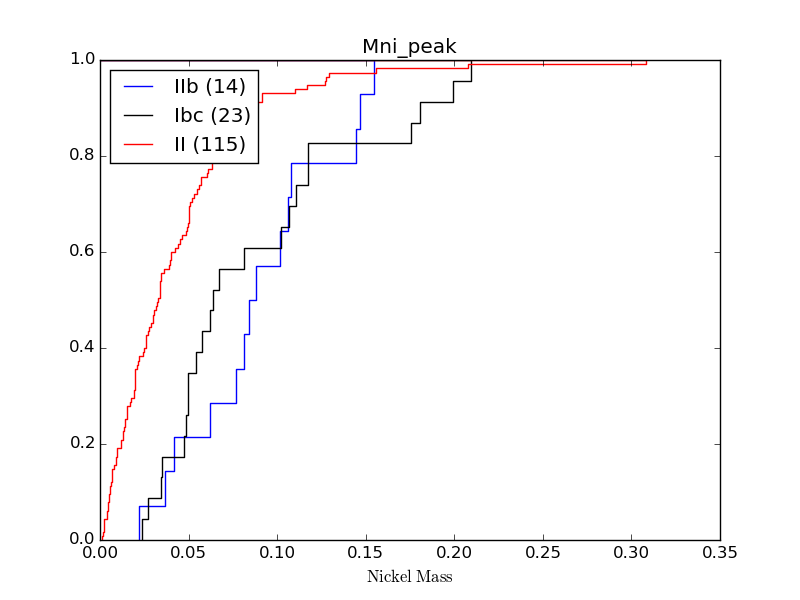
\includegraphics[width=\linewidth]{plots/Mni_peak_hist_IIb-Ibc.png}
\caption{Final distribution of 56Ni, using the Arnett's rule, for our BVRIYJH sample of SNe, grouping all types Ibc together. \label{fig:hist_all}}
\end{figure}

\begin{figure}[ht!]
 \centering
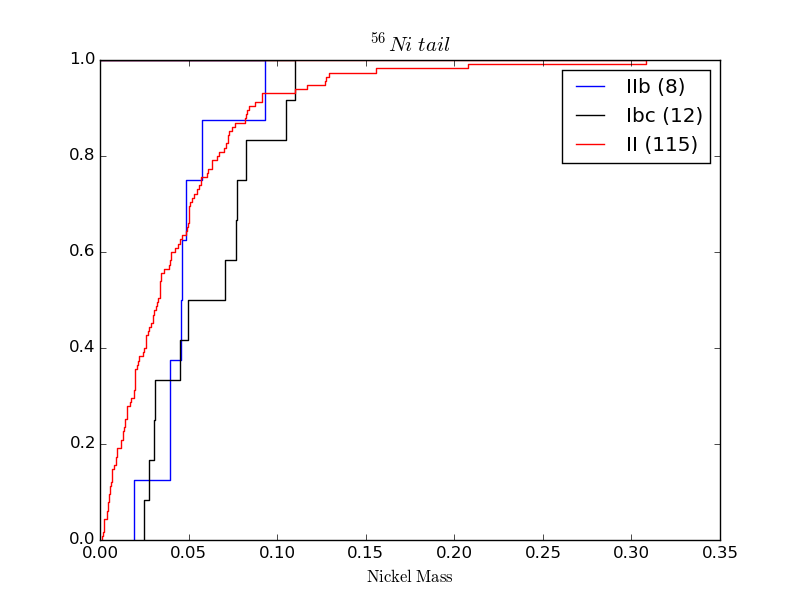
\includegraphics[width=\linewidth]{plots/Mni_tail_hist_IIb-Ibc.png}
\caption{Final distribution of 56Ni, using the tail bolometric luminosity, for our BVRIYJH sample of SNe, grouping all types Ibc together. \label{fig:hist_all}}
\end{figure}


\section{Discussion and conclusions}

\label{sec:conclusions}
%______________________________________________________________



\begin{acknowledgements}
      
\end{acknowledgements}

% WARNING
%-------------------------------------------------------------------
% Please note that we have included the references to the file aa.dem in
% order to compile it, but we ask you to:
%
% - use BibTeX with the regular commands:
%   \bibliographystyle{aa} % style aa.bst
%   \bibliography{Yourfile} % your references Yourfile.bib
%
% - join the .bib files when you upload your source files
%-------------------------------------------------------------------

\begin{thebibliography}{}
\bibitem[Anderson(2019)]{2019A&A...628A...7A} Anderson, J.~P.\ 2019, \aap, 628, A7
  
\end{thebibliography}

%-------------------------------------------------------------
%                                             Simple A&A Table
%-------------------------------------------------------------

\begin{table*}
\centering
\scriptsize
\caption{Sample of SNe\label{tab:table}}
\begin{tabular}{cccccccccccc}
\hline
{SN}&{Type}&{Host}&{Host redshift}&{Host $d_L$}&{$E(B-V)$}&{$t_0$}&{t-discovery}&{mag-discovery}&{t-non detection}&{m-non detection}\\
\hline
SN1993J&IIb&"M81"&-0.00011&3.63&0.071&49073.5&49074.89&12.0&49072.89&14.0\\ 
SN1994I&Ic&"M51"&0.0015&8.31&0.03&49438.5&49444.169&13.5&49443.25&14.0\\ 
SN1996cb&IIb&"NGC3510"&0.0024&9.77&0.12&50429.0&50432.707&16.5&50427.0&99.0\\ 
SN1998bw&Ic-GRB&"ESO184-G82"&0.0087&35.65&0.052&50928.89&None&99.0&None&99.0\\ 
SN1999dn&Ib&"NGC7714"&0.0093&38.547&0.052&51406.0&51409.759&16.0&51400.0&18.0\\ 
SN1999ex&Ibc&"IC5179"&0.0114&48.75&0.02&51480.0&51491.509&None&51476.58&19.0\\ 
SN2001ig&IIb&"NGC7424"&0.00313&12.59&0.011&52246.0&52253.0&14.5&None&99.0\\ 
SN2002ap&Ic-BL&"M74"&0.0022&7.94&0.071&52302.0&52303.39&14.5&52299.0&18.0\\ 
SN2003jd&Ic-BL&"PGC71157"&0.019&76.9&0.06&52932.7&52937.2&16.5&52928.2&19.0\\ 
SN2003dh&Ic-GRB&"A104450+2131"&0.168&695.0&0.025&52727.5&None&99.0&None&99.0\\ 
SN2003bg&IIb&"MCG-05-10-15"&0.0046&21.677&0.02&52695.0&52695.7&15.0&52585.0&18.0\\ 
SN2003lw&Ic-GRB&"A080230-3951"&0.1055&475.0&0.9&52976.916&None&99.0&None&99.0\\ 
SN2004ao&Ib&"UGC10862"&0.00564&26.91&0.0893&None&56723.54&14.9&56548.21&19.0\\ 
SN2004ex&IIb&"NGC0182"&0.01755&70.6&0.0196&53287.9&53289.34&17.7&53272.27&19.0\\ 
SN2004ew&Ib&"ESO153G017"&0.021761&90.5&0.027&53260.21&53287.92&17.5&53260.21&18.1\\ 
SN2004gq&Ib&"NGC1832"&0.006468&25.1&0.0627&53346.87&53350.36&15.5&53343.38&19.5\\ 
SN2004gv&Ib&"NGC0856"&0.019973&79.6&0.0276&53345.27&53352.67&17.6&53337.74&18.6\\ 
SN2004gt&Ic&"NGC4038"&0.005477&23.2&0.0398&53342.834&53351.08&14.9&53136.25&15.7\\ 
SN2004ff&IIb&"ESO-552-G040"&0.0226&92.7&0.029&53297.66&53308.4&18.0&53291.41&19.0\\ 
SN2004fe&Ic&"NGC0132"&0.017895&72.1&0.021&53306.74&53308.29&18.1&53300.28&19.0\\ 
SN2004aw&Ic&"NGC3997"&0.016&72.77&0.018&53081.2&53083.9&17.1&53078.0&18.5\\ 
SN2004dn&Ic&"UGC2069"&0.0126&51.4&0.0412&53205.419&53215.419&18.5&53027.209&19.5\\ 
SN2004ge&Ic&"UGC3555"&0.01612&67.0&0.0752&None&53326.459&18.3&53323.45&19.5\\ 
SN2004gk&Ic&"IC3311"&0.0&17.0&0.0247&None&53334.5&13.3&53168.169&17.9\\ 
SN2004dk&Ib&"NGC6118"&0.00525&23.0&0.1354&None&53218.19&17.6&53215.2&18.0\\ 
SN2005aw&Ic&"IC4837A"&0.009498&41.5&0.054&53445.67&53453.27&15.3&53436.32&17.9\\ 
SN2005az&Ic&"NGC4961"&0.00845&39.0&0.0097&None&53457.209&17.4&53449.229&17.4\\ 
SN2005em&Ic&"IC0307"&0.025981&105.0&0.0848&53638.16&53640.44&18.1&53615.43&19.5\\ 
SN2005ek&Ic&"UGC2526"&0.01655&66.6&0.1788&None&53637.53&17.5&53631.509&19.0\\ 
SN2005eo&Ic&"UGC4132"&0.01741&85.0&0.0581&None&53640.189&18.3&53464.149&19.5\\ 
SN2005mf&Ic&"UGC4798"&0.02676&113.0&0.0153&None&53729.669&17.4&53717.0&18.5\\ 
SN2005Q&IIb&"ESO-244-G031"&0.02243&90.8&0.0055&53385.7&53398.8&17.2&53369.81&20.5\\ 
SN2005bj&IIb&"MGC+03-43-005"&0.022179&99.8&0.0767&53452.08&53471.1&17.7&53191.0&19.5\\ 
SN2005hg&Ib&"UGC1394"&0.02131&86.0&0.0901&None&53668.27&18.6&53663.24&19.5\\ 
SN2005hl&Ib&"A205519+0032"&0.023&100.4&0.073&53628.26&53625.0&18.9&None&99.0\\ 
SN2005hm&Ib&"A213900-0101"&0.035&151.6&0.048&53641.96&53628.0&20.6&None&99.0\\ 
SN2005kr&Ic-BL&"A030829+0053"&0.134&627.0&0.087&53670.2&53677.0&22.1&None&99.0\\ 
SN2005ks&Ic-BL&"A213756-0001"&0.099&451.0&0.05&53687.82&53678.0&22.5&None&99.0\\ 
SN2005kz&Ic-BL&"PGC62678"&0.027&115.0&0.054&None&53705.03&18.7&53675.0&20.0\\ 
SN2005kl&Ic&"NGC4369"&0.003485&21.57&0.0219&53686.14&53696.14&14.6&None&99.0\\ 
SN2005nb&Ic-BL&"UGC7230"&0.02377&108.0&0.03&53711.0&53721.379&17.2&None&99.0\\ 
SN2006T&IIb&"NGC3054"&0.008091&31.6&0.195&53757.64&53766.0&17.2&53751.95&18.0\\ 
SN2006F&Ib&"NGC935"&0.0139&55.0&0.19&None&53746.78&17.3&53695.0&18.5\\ 
SN2006dn&Ib&"UGC12188"&0.017062&70.0&0.113&None&53912.49&18.7&53895.49&18.5\\ 
SN2006ep&Ib&"NGC214"&0.015134&61.9&0.225&53975.49&53977.35&17.8&53973.64&19.0\\ 
SN2006fo&Ib&"UGC02019"&0.020698&82.7&0.025&53983.36&53994.0&18.2&None&99.0\\ 
SN2006aj&Ic-GRB&"A032139+1652"&0.033&132.4&0.097&53784.14861&None&99.0&None&99.0\\ 
SN14475&Ic-BL&"SDSSJ222430.86+0012&0.149&705.0&0.072&54028.05&None&99.0&None&99.0\\ 
SN2006ba&IIb&"NGC2980"&0.01908&82.7&0.15&53801.11&53813.81&18.4&53771.04&18.8\\ 
SN2006bf&IIb&"UGC08093"&0.023867&108.0&0.174&53797.65&53821.35&17.7&53741.0&19.3\\ 
SN2006el&IIb&"UGC12188"&0.0171&70.7&0.303&None&53972.28&18.2&53965.319&19.4\\ 
SN2006dn&Ib&"UGC12188"&0.0171&70.7&0.303&None&53891.45&17.8&53881.49&18.7\\ 
SN2006ep&Ib&"NGC0214"&0.015134&61.9&0.032&53975.49&53977.35&17.8&53973.64&19.0\\ 
SN2006gi&Ib&"NGC3147"&0.00935&43.65&0.122&53977.5&53996.79&16.3&53889.0&19.0\\ 
SN2006jc&Ib-n&"UGC4904"&0.005484&25.0&0.0173&None&54017.7519&13.8&54000.0&19.0\\ 
SN2006jo&Ib&"A012314-0019"&0.077&345.8&0.492&54001.54&54008.0&21.1&None&99.0\\ 
SN2006lc&Ib&"NGC7364"&0.016228&59.2&0.41&54014.74&54029.0&20.2&None&99.0\\ 
SN2006ir&Ic&"KUG2302+073/PGC0853&0.02&82.2&0.04&53988.26&54001.29&16.9&None&99.0\\ 
SN2006ab&Ic&"PGC10652"&0.01652&68.0&0.489&None&53775.18&18.0&53759.16&18.6\\ 
SN2006fe&Ic&"SDSSJ205209.10-0030&0.07&316.3&0.098&53954.0&53974.0&21.0&None&99.0\\ 
SN2006nx&Ic-BL&"A033330-0040"&0.137&642.0&0.108&54050.21&54040.0&22.1&None&99.0\\ 
SN2006ck&Ic&"UGC8238"&0.02439&111.0&0.0245&None&53875.54&17.4&53823.7&18.0\\ 
SN2006ld&Ib&"UGC348"&0.013939&55.0&0.0144&None&54027.29&16.0&53998.0&20.0\\ 
SN2006lv&Ib&"UGC6517"&0.008305&40.0&0.0245&54026.0&54036.1239&17.0&None&99.0\\ 
SN2007C&Ib&"NGC4981"&0.005604&21.0&0.47&54095.44&54107.86&15.9&54092.87&18.5\\ 
SN2007Y&Ib&"NGC1187"&0.004637&18.4&0.019&54145.0&54146.77&17.5&54082.85&18.0\\ 
SN2007kj&Ib&"NGC7803"&0.017899&72.5&0.07&54363.61&54375.6&17.4&54363.61&19.0\\ 
SN2007nc&Ib&"A000109+0104"&0.087&393.9&0.081&54400.04&54381.0&22.5&None&99.0\\ 
SN2007uy&Ib&"NGC2770"&0.0065&31.33&0.652&54462.33&54465.67&17.2&54452.0&18.0\\ 
SN2007gr&Ic&"NGC1058"&0.0017&9.289&0.085&54325.0&54327.509&13.8&54322.43&18.9\\ 
SN2007ag&Ic&"UGC05392"&0.020711&91.0&0.026&54155.0&54166.29&18.0&54155.0&19.4\\ 
SN2007hn&Ic&"NPM1G-04.0556"&0.0273&113.3&0.007&54340.82&54343.2&18.6&None&99.0\\ 
SN2007rz&Ic&"NGC1590"&0.01299&52.2&0.177&54426.5&54442.4&16.9&54423.41&19.5\\ 
SN2007ag&Ic&"UGC5392"&0.0207&91.0&0.0258&54155.0&54166.29&18.0&54155.0&19.4\\ 
SN2007qv&Ic&"A223507-0106"&0.095&433.5&0.048&None&54408.0&21.9&None&99.0\\ 
SN2007qx&Ic&"A002741+0113"&0.08&363.3&0.023&None&54409.0&22.4&None&99.0\\ 
SN2007sj&Ic&"A001039-0003"&0.039&170.1&0.032&None&54421.0&21.2&None&99.0\\ 
SN2007D&Ic-BL&"UGC2653"&0.0231&93.0&0.335&54099.0&54109.02&18.2&53710.0&19.4\\ 
SN2007ms&Ic&"A203218-0100"&0.039&171.0&0.184&54368.79&53626.0&20.7&None&99.0\\ 
SN2007ru&Ic-BL&"UGC12381"&0.01546&67.6&0.26&54429.5&54431.89&17.5&54426.16&18.9\\ 
SN2007ce&Ic-BL&"ANON"&0.04599&210.0&0.02&None&54224.14&17.4&54214.12&17.8\\ 
SN2007bg&Ic-BL&"Anon"&0.03459&150.0&0.018&None&54206.149&17.7&54196.149&18.2\\ 
SN2007I&Ic-BL&"PGC1114807"&0.021638&100.0&0.025&None&54114.439&18.0&54076.459&19.2\\ 
SN2007cl&Ic&"NGC6479"&0.02218&95.5&0.02&54233.0&54243.339&17.6&None&99.0\\ 
SN2008gc&Ib&"B020852.09-5400"&0.0492&207.6&0.165&54724.45&54742.16&17.4&54651.28&18.0\\ 
SN2008aq&IIb&"MCG-02-33-020"&0.007972&26.9&0.04&54510.79&54523.94&16.3&54506.97&19.1\\ 
SN2008ax&IIb&"NGC4490"&0.0019&9.204&0.3&54528.3&54528.45&16.1&54528.2&18.5\\ 
SN2008D&Ib&"NGC2770"&0.0065&31.33&0.65&54474.5&54476.419&17.5&54467.419&19.6\\ 
SN2008hh&Ic&"IC0112"&0.01941&77.7&0.044&54780.69&54789.12&16.6&54759.0&19.2\\ 
SN2008hw&Ic-GRB&"ANON"&0.5295&2270.0&0.0138&54746.2249&None&99.0&None&99.0\\ 
SN2008bo&IIb&"NGC6643"&0.00495&20.6&0.05&54546.0&54556.919&16.6&None&99.0\\ 
SN2009jf&Ib&"NGC7479"&0.0079&33.728&0.162&55099.0&55101.33&18.0&55097.319&19.2\\ 
SN2009bb&Ic&"NGC3278"&0.00988&39.8&0.58&54909.1&54911.109&17.0&54909.2&18.0\\ 
SN2009K&IIb&"NGC1620"&0.011715&44.1&0.111&54843.57&54844.07&14.9&54842.08&18.0\\ 
SN2009Z&IIb&"A140153-0120"&0.02513&108.1&0.04&54860.04&54864.53&18.1&None&19.4\\ 
SN2009mg&IIb&"ESO121-G26"&0.0076&32.7&0.14&55168.0&55172.9&17.3&55125.05&18.8\\ 
SN2009iz&Ib&"UGC02175"&0.01419&58.6&0.0729&55083.0&55093.52&18.2&55081.45&18.2\\ 
SN2009ca&Ic-BL&"A212622-4051"&0.0956&417.5&0.03&54915.36&54920.37&17.1&54766.19&18.5\\ 
SN2009dt&Ic&"IC5169"&0.010374&44.4&0.0145&54945.84&54949.33&17.2&54942.36&19.0\\ 
SN2009dp&Ic&"NGC6912"&0.023244&100.0&0.061&54939.0&54944.1&17.7&54923.1&18.5\\ 
SN2009nz&Ic-GRB&"ANON"&0.49&2754.2&0.035&55162.976&None&99.0&None&99.0\\ 
SN2009er&Ib-pec&"SDSSJ1539+2426h"&0.035024&150.0&0.039&None&54973.99&17.7&54912.0&19.5\\ 
SN2010O&Ib&"NGC3690"&0.0104&44.8&0.016&55203.2&55214.2&16.55&None&99.0\\ 
SN2010as&IIb&"NGC6000"&0.0073&27.164&0.57&55270.75&55274.219&15.5&55267.33&17.5\\ 
SN2010bh&Ic-GRB&"A071031-5615"&0.059&244.34&0.26&55271.5311&None&99.0&None&99.0\\ 
SN2010ah&Ic-BL&"A114403+5541"&0.0498&218.0&0.012&None&55250.5038&18.8&55246.439&20.9\\ 
SN2010ay&Ic-BL&"A123527+2704"&0.0671&297.9&0.017&55248.29&55260.45&18.2&55244.45&18.3\\ 
SN2010ma&Ic-GRB&"A004855-3433"&0.55185&3022.0&0.017&55549.68603&None&99.0&None&99.0\\ 
SN2011hs&IIb&"IC5267"&0.0057&24.1&0.171&55871.5&55877.4759&15.5&55843.574&18.7\\ 
SN2011fu&IIb&"UGC1626"&0.019&74.47&0.083&55824.0&55824.78&16.1&55783.0&18.8\\ 
SN2011dh&IIb&"M51"&0.002&7.87&0.085&55712.5&55712.89&14.0&55712.2749&21.44\\ 
SN2011bm&Ic&"IC3918"&0.022&97.7&0.064&55643.5&55646.5&18.71&55643.0&20.8\\ 
SN2011ei&IIb&"NGC6925"&0.00931&28.5&0.24&55737.0&55767.43&18.0&55735.58&19.1\\ 
SN2011kl&Ic-GRB&"A005722-4648"&0.677&4200.0&0.0145&55904.3&None&99.0&None&99.0\\ 
SN2012P&IIb&"NGC5806"&0.00449&26.8&0.33&55932.5&55936.48&17.0&55931.0&99.0\\ 
SN2012ap&Ic&"NGC1729"&0.012&48.97&0.445&55962.0&55967.229&17.3&55962.2&18.7\\ 
SN2012bz&Ic-GRB&"A090738+1401"&0.28&1153.5&0.037&56029.0&None&99.0&None&99.0\\ 
SN2012au&Ib&"NGC4790"&0.00448&23.5&0.063&None&55988.359&18.2&55979.459&19.4\\ 
SN2012aa&Ibc&"ANON"&0.083&380.2&0.088&55955.54&55955.56&17.7&55693.0&19.1\\ 
SNPTF12gzk&Ic-BL&"SDSSJ221241.53+0030&0.0137&57.8&0.0429&56130.549&56132.29&20.66&56127.0&21.6\\ 
SN2013ge&Ibc&"NGC3287"&0.0044&23.66&0.067&56602.6&56604.796&16.8&56597.7879&18.5\\ 
SN2013df&IIb&"NGC4414"&0.0024&21.37&0.097&56447.299&56450.87&14.4&56437.0&18.5\\ 
SN2013cq&Ic-GRB&"A113232+2741"&0.34&1729.816&0.07&56409.3&None&99.0&None&99.0\\ 
SN2013cu&IIb&"UGC9379"&0.026&111.17&0.011&56414.93&56415.18&20.1&56412.0&21.22\\ 
SNiPTF13bvn&Ib&"NGC5806"&0.0045&23.88&0.0715&56458.669&56459.24&18.6&56458.24&21.7\\ 
SN2013dx&Ic-GRB&"A142914+1546"&0.145&709.0&0.036&0.0&None&99.0&None&99.0\\ 
SN2014ad&Ic-BL&"PGC3762"&0.0057&26.44&0.045&56724.5&56728.399&15.7&56722.37&19.0\\ 
SN2014L&Ic&"NGC4254"&0.00802&14.0&0.04&56680.0&56681.85&17.9&None&99.0\\ 
SNiPTF15dtg&Ic&"ANON"&0.0524&232.0&0.0544&57332.948&57333.431&19.63&57332.433&20.46\\ 
SN2015as&IIb&"UGC5460"&0.00365&19.2&0.008&57332.0&57335.0&17.59&None&99.0\\ 
SN2016coi&Ic&"UGC11868"&0.00364&17.2&0.08&nan&57535.549&15.7&57529.54&16.7\\ 
SN2016jca&Ic-GRB&"ANON"&0.1475&700.0&0.0281&57741.7879&None&99.0&None&99.0\\ 
SN2016gkg&IIb&"NGC613"&0.00494&26.0&0.0166&57651.1875&57651.223&19.0&57651.2&19.4\\ 
SN2017ein&Ic&"NGC3938"&0.002698&17.0&0.0187&57897.6&57898.77&17.7&57896.77&19.9\\ 
SN2017czd&IIb&"UGC9567"&0.00835&32.0&0.02&57854.5&57855.7&15.5&57845.75&19.0\\ 
SNiPTF17cw&Ic-BL&"ANON"&0.093&429.0&0.0166&None&57760.0&19.55&57728.0&99.0\\ 
\end{tabular}
\end{table*}


\end{document}


%-------------------------------------------------------------
%               Appendices have to be placed at the end, after
%                                        \end{thebibliography}
%-------------------------------------------------------------
\end{thebibliography}

\begin{appendix} %First appendix
\section{Background galaxy number counts and shear noise-levels}
Because the optical images used in this analysis...
\begin{figure*}%f1
\includegraphics[width=10.9cm]{1787f23.eps}
\caption{Shown in greyscale is a...}
\label{cl12301}
\end{figure*}

In this case....
\begin{figure*}
\centering
\includegraphics[width=16.4cm,clip]{1787f24.ps}
\caption{Plotted above...}
\label{appfig}
\end{figure*}

Because the optical images...

\section{Title of Second appendix.....} %Second appendix
These studies, however, have faced...
\begin{table}
\caption{Complexes characterisation.}\label{starbursts}
\centering
\begin{tabular}{lccc}
\hline \hline
Complex & $F_{60}$ & 8.6 &  No. of  \\
...
\hline
\end{tabular}
\end{table}

The second method produces...
\end{appendix}
%
%
\end{document}

%
%-------------------------------------------------------------
%          For the appendices, table longer than a single page
%-------------------------------------------------------------

% Table will be print automatically at the end of the document, 
% after the whole appendices

\begin{appendix} %First appendix
\section{Background galaxy number counts and shear noise-levels}

% In the appendices do not forget to put the counter of the table 
% as an option

\longtab[1]{
\begin{longtable}{lrcrrrrrrrrl}
\caption{Line data and abundances ...}\\
\hline
\hline
Def & mol & Ion & $\lambda$ & $\chi$ & $\log gf$ & N & e &  rad & $\delta$ & $\delta$ 
red & References \\
\hline
\endfirsthead
\caption{Continued.} \\
\hline
Def & mol & Ion & $\lambda$ & $\chi$ & $\log gf$ & B & C &  rad & $\delta$ & $\delta$ 
red & References \\
\hline
\endhead
\hline
\endfoot
\hline
\endlastfoot
A & CH & 1 &3638 & 0.002 & $-$2.551 &  &  &  & $-$150 & 150 &  Jorgensen et al. (1996) \\                    
\end{longtable}
}% End longtab
\end{appendix}

%-------------------------------------------------------------
%                   For appendices and landscape, large table:
%                    in the preamble, use: \usepackage{lscape}
%-------------------------------------------------------------

\begin{appendix} %First appendix
%
\longtab[1]{
\begin{landscape}
\begin{longtable}{lrcrrrrrrrrl}
...
\end{longtable}
\end{landscape}
}% End longtab
\end{appendix}

%%%% End of aa.dem
